\documentclass[11pt, titlepage]{article}
% Common packages/environments to remove clutter

% Packages
\usepackage[utf8]{inputenc}
\usepackage{amsmath, amsfonts, amssymb, amsthm, enumitem, tikz, import, mathtools}
\usepackage[
  top=2cm,
  bottom=2cm,
  left=3cm,
  right=3cm,
  headheight=17pt,
  includehead, includefoot,
  heightrounded,
]{geometry}

% Problem environment
\newtheoremstyle{emptyplain}
    {}          % default space above
    {}          % default space below
    {}          % default body font
    {}          % no indent
    {\bfseries} % head font
    {.}         % punctuation after theorem head
    { }         % space after theorem head
    {#3}
\theoremstyle{emptyplain}
\newtheorem*{problem}{}

% Solution Environment
\newenvironment{solution}{
  \begin{proof}[Solution]
    \vspace{-2px}
    \setlength{\parskip}{4px}
    \setlength{\parindent}{0px}
}{
\end{proof}
}

\usepackage{fancyhdr, float}
\usepackage[
    top=2cm,
    bottom=2cm,
    left=3cm,
    right=3cm,
    headheight=17pt,
    includehead, includefoot, heightrounded,
]{geometry}

% Phase line command
\newcommand*{\TickSize}{2pt}%

\newcommand*{\AxisMin}{0}%
\newcommand*{\AxisMax}{0}%

\newcommand*{\DrawHorizontalPhaseLine}[4][]{%
    % #1 = axis tick labels
    % #2 = right arrows positions as CSV
    % #3 = left arrow positions as CSV
    \gdef\AxisMin{0}%
    \gdef\AxisMax{0}%
    \edef\MyList{#2}% Allows for #1 to be both a macro or not
    \foreach \X in \MyList {
        \draw  (\X,\TickSize) -- (\X,-\TickSize) node [below] {$\X$};
        \ifnum\AxisMin>\X
            \xdef\AxisMin{\X}%
        \fi
        \ifnum\AxisMax<\X
            \xdef\AxisMax{\X}%
        \fi
    }

    \edef\MyList{#3}% Allows for #2 to be both a macro or not
    \foreach \X in \MyList {% Right arrows
        \draw [->] (\X-0.1,0) -- (\X,0);
        \ifnum\AxisMin>\X
            \xdef\AxisMin{\X}%
        \fi
        \ifnum\AxisMax<\X
            \xdef\AxisMax{\X}%
        \fi
    }

    \edef\MyList{#4}% Allows for #3 to be both a macro or not
    \foreach \X in \MyList {% Left arrows
        \draw [<-] (\X-0.1,0) -- (\X,0);
        \ifnum\AxisMin>\X
            \xdef\AxisMin{\X}%
        \fi
        \ifnum\AxisMax<\X
            \xdef\AxisMax{\X}%
        \fi
    }

    \draw  (\AxisMin-1,0) -- (\AxisMax+1,0) node [right] {#1};
}

% Header
\pagestyle{fancy}
\fancyhf{}
\lhead{Math 2552 Final Exam Makeup Part A}
\rhead{Akash Narayanan}

% Opening
\title{Math 2552 Final Exam Makeup Part A}
\author{Akash Narayanan}
\date{May 7, 2021}

\begin{document}
    \maketitle

    \begin{enumerate}
        % Problem 1
        \item (4 points) Solve the IVP.
        \[
        y' = 9t^2y^2, \quad y(0) = \frac{1}{2}
        \]

        \begin{solution}
            This is a separable differential equation so we start by rewriting it as
            \[
            \frac{1}{y^2} dy = 9t^2 dt
            \]
            Integrating both sides yields
            \[
            -\frac{1}{y} = 3t^3 + C
            \]
            We use the initial condition to solve for the constant:
            \begin{align*}
                -\frac{1}{\frac{1}{2}} &= 3(0)^3 + C \\
                C &= -2
            \end{align*}
            Thus, we have
            \[
            -\frac{1}{y} = 3t^3 - 2
            \]
            or
            \[
            y = \frac{1}{2 - 3t^3}
            \]
        \end{solution}

        \pagebreak

        % Problem 2
        \item (10 points) Solve the differential equation using the method of undetermined coefficients.
        \[
        y'' - 5y' + 4y = 68\cos t - 12e^t
        \]

        \begin{solution}
            We begin by finding the general solution to the homogeneous equation.
            The characteristic equation is $r^2 - 5r + 4$ which has zeroes at $r = 1, 4$.
            Then the general solution to the homogeneous equation is
            \[
            y_h(t) = c_1 e^{t} + c_2 e^{4t}
            \]
            A first guess for the form of the particular solution is
            \[
            y_p = A \sin t + B \cos t + C e^{t}
            \]
            but the third term is a solution to the homogeneous equation so we multiply it by a factor of $t$.
            Differentiating gives
            \begin{align*}
                y_p &= A \sin t + B \cos t + Ct e^{t} \\
                y'_p &= A \cos t - B \sin t + (Ct + C) e^{t} \\
                y''_p &= -A \sin t - B \cos t + (Ct + 2C) e^{t}
            \end{align*}
            Plugging these into the differential equation (and simplifying) yields
            \[
                (3A + 5B) \sin t + (3B - 5A) \cos t - 3C e^{t} = 68 \cos t - 12 e^{t}
            \]
            Matching coefficients, we have the system of equations
            \begin{align*}
                3A + 5B &= 0 \\
                3B - 5A &= 68
            \end{align*}
            which has the solution $A = -10, B = 6$.
            We also find $C = 4$.
            Thus, the solution to the differential equation is the sum of the homogeneous solution and the particular solution
            \[
            y = c_1 e^{t} + c_2 e^{4t} - 10 \sin t + 6 \cos t + 4t e^{t}
            \]
        \end{solution}

        \pagebreak

        % Problem 3
        \item (10 points) Consider the homogeneous linear system of differential equations.
        \[
        \vec{x}' = A\vec{x} =
        \begin{pmatrix}
            5 & \frac{1}{2} \\
            -\frac{1}{2} & 4
        \end{pmatrix} \vec{x}, \quad
        \vec{x} = \vec{x}(t) =
        \begin{pmatrix}
            x_1(t) \\
            x_2(t)
        \end{pmatrix}
        \]

        \begin{enumerate}[label={(\alph*)}]
            \item (2 points) Determine the eigenvalues of $A$. Show your work.

            \item (5 points) Express the general solution of the system in terms of real valued functions.

            \item (3 points) Sketch the phase portrait of the system.
            Please include the eigenspaces in your sketch, indicate the direction of motion of your solution curves and eigenspaces, and do not forget to label your axes.
        \end{enumerate}

        \begin{solution}
            We calculate the determinant of $A - \lambda I$.
            \[
            \det
            \begin{pmatrix}
                5 - \lambda & \frac{1}{2} \\
                -\frac{1}{2} & 4 - \lambda
            \end{pmatrix} = \lambda^2 - 9\lambda + \frac{81}{4} = \left( \lambda - \frac{9}{2} \right)^2 = 0
            \]
            Thus, the only eigenvalue is $\lambda = \frac{9}{2}$ with multiplicity 2.

            To calculate the associated eigenvector, we set $\lambda = \frac{9}{2}$ and solve $(A - \lambda I) \vec{v}_1 = 0$.
            \[
            \begin{pmatrix}
                \frac{1}{2} & \frac{1}{2} \\
                -\frac{1}{2} & \frac{-1}{2}
            \end{pmatrix} \vec{v}_1 =
            \begin{pmatrix}
                0 \\
                0
            \end{pmatrix}
            \]
            which has the solution
            \[
            \vec{v}_1 =
            \begin{pmatrix}
                1 \\
                -1
            \end{pmatrix}
            \]

            To find a second solution, we solve $(A - \lambda I) \vec{v}_2 = \vec{v}_1$.
            \[
            \begin{pmatrix}
                \frac{1}{2} & \frac{1}{2} \\
                -\frac{1}{2} & \frac{-1}{2}
            \end{pmatrix} \vec{v}_2 =
            \begin{pmatrix}
                1 \\
                -1
            \end{pmatrix}
            \]
            which has the solution
            \[
            \vec{v}_2 =
            \begin{pmatrix}
                1 \\
                1
            \end{pmatrix}
            \]
            Then the general solution to the system of differential equations is
            \[
            \vec{x}(t) = c_1 e^{\frac{9}{2}t}
            \begin{pmatrix}
                -1 \\
                1
            \end{pmatrix}
            + c_2 e^{\frac{9}{2}t}
            \begin{pmatrix}
                t + 1 \\
                1 - t
            \end{pmatrix}
            \]

            The phase portrait has one eigenvector which is denoted by the red line and the solution curves point away from the origin.
            \begin{figure}[H]
                \centering
                \def\svgwidth{0.8\columnwidth}
                \import{media/}{phasePortrait9.pdf_tex}
            \end{figure}
        \end{solution}

        \pagebreak

        % Problem 4
        \item (10 points) Consider the differential equation $\frac{dy}{dt} = (y + 2)(y - 3)$, where $y$ is a real function of $t$, and $t \geq 0$, and $k > 0$.

        \begin{enumerate}[label={(\alph*)}]
            \item State the critical points of the differential equation.

            \item Draw the phase line, and determine whether the critical points (if any) are stable, semi-stable, or unstable. Show your work.

            \item Determine where $y$ is concave up and concave down for $y \in \mathbb{R}$. Show your work.

            \item Use results from parts (a), (b), and (c) to sketch several solution curves in the $ty$-plane for $t \geq 0$.
        \end{enumerate}

        \begin{solution}
            The critical points are points where the derivative is equal to zero, which can be found by setting each factor to zero.
            We find critical points at $y = -2$ and $y = 3$.
            We can classify the equilibrium points by evaluating the sign of the derivative over various intervals, expressed in the following table.
            \begin{center}
                \begin{tabular}{ |c|c| }
                    \hline
                    $y$ & $dy / dt$ \\
                    \hline
                    $y < -2$ & $dy / dt > 0$ \\
                    \hline
                    $-2 < y < 3$ & $dy / dt < 0$ \\
                    \hline
                    $3 < y$ & $dy / dt > 0$ \\
                    \hline
                \end{tabular}
            \end{center}
            With this information, we can draw the phase line.

            \begin{figure}[h]
                \centering
                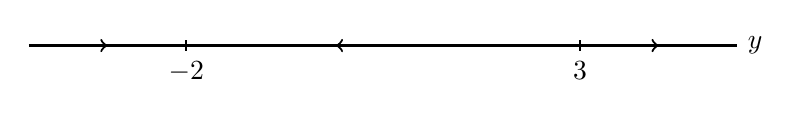
\begin{tikzpicture}[thick]
                    [scale=1.5]
                    \DrawHorizontalPhaseLine[$y$]{-2, 3}{-3, 4}{0}
                \end{tikzpicture}
            \end{figure}
            This makes it easy to see that $y = -2$ is stable while $y = 3$ is unstable.

            We find
            \[
            \frac{d^2y}{dt^2} = \frac{d}{dt} (y+2)(y - 3) = \frac{d}{dy} (y + 2)(y  - 3) \cdot \frac{dy}{dt} = (2y - 1) \cdot \frac{dy}{dt}
            \]
            We know $y$ is concave up when $y''$ is positive, or when both factors in the above equation have the same sign.
            We can organize this into a table.
            \begin{center}
                \begin{tabular}{ |c|c|c| }
                    \hline
                    $y$ & $2y - 1$ & Concavity \\
                    \hline
                    $y < -2$ & $2y - 1 < 0$ & Concave down \\
                    \hline
                    $-2 < y < \frac{1}{2}$ & $2y - 1 < 0$ & Concave up \\
                    \hline
                    $\frac{1}{2} < y < 3$ & $2y - 1 > 0$ & Concave down \\
                    \hline
                    $3 < y$ & $2y - 1$ & Concave up \\
                    \hline
                \end{tabular}
            \end{center}
            Thus, $y$ is concave down on $(-\infty, -2) \cup (1 / 2, 3)$ and concave up on $(-2, 1 / 2) \cup (3, \infty)$.

            The solution curves can vary based on the value of $y(0)$ (I apologize for any abrupt changes, the curve should be differentiable everywhere along the curve).
            \begin{figure}[H]
                \centering
                \def\svgwidth{0.8\columnwidth}
                \import{media/}{phasePortrait4.pdf_tex}
            \end{figure}
        \end{solution}

        \pagebreak

        % Problem 5
        \item (5 points) The position of a moving object, $y(t)$, for time $t \geq 0$ satisfies the IVP
        \[
        y'' + y' - 2y = 0, \quad y = y(t)
        \]

        \begin{enumerate}[label={(\alph*)}]
            \item Express the differential equation in the IVP as a first-order system in the form $\vec{x}' = A\vec{x}$.

            \item Solve the DE using any method you like. Show your work.

            \item Sketch the trajectory of the object for $t \geq 0$ in the phase plane.
            Please include the eigenspaces of $A$ in your sketch,
            indicate the direction of motion on your solution curves and eigenspaces,
            and do not forget to label your axes.
        \end{enumerate}

        \begin{solution}
            To express the differential equation as a first-order system, we set $x_1 = y$ and $x_2 = y'$.
            Then we find
            \begin{align*}
                x_1' &= y' = x_2 \\
                x_2' &= y'' = 2y - y' = 2x_1 - x_2
            \end{align*}
            so the system can be expressed as $\vec{x}' = A\vec{x}$ where
            \[
            A =
            \begin{pmatrix}
                0 & 1 \\
                2 & -1
            \end{pmatrix}
            \]

            To solve the differential equation, we find the eigenvalues of the matrix.
            \begin{gather*}
                \det
                \begin{pmatrix}
                    -\lambda & 1 \\
                    2 & -1 - \lambda
                \end{pmatrix} = \lambda^2 + \lambda - 2 = (\lambda + 2)(\lambda - 1) = 0 \\
                \Longrightarrow \lambda = -2, 1
            \end{gather*}
            Now we find the associated eigenvectors by solving $(A - \lambda I) \vec{v} = 0$.
            \begin{gather*}
                \begin{pmatrix}
                    2 & 1 \\
                    2 & 1
                \end{pmatrix} \vec{v}_1 =
                \begin{pmatrix}
                    0 \\
                    0
                \end{pmatrix} \\
                \Longrightarrow
                \vec{v}_1 =
                \begin{pmatrix}
                    1 \\
                    -2
                \end{pmatrix} \\
                \begin{pmatrix}
                    -1 & 1 \\
                    2 & -2
                \end{pmatrix} \vec{v}_2 =
                \begin{pmatrix}
                    0 \\
                    0
                \end{pmatrix} \\
                \Longrightarrow
                \vec{v}_2 =
                \begin{pmatrix}
                    1 \\
                    1
                \end{pmatrix}
            \end{gather*}
            Since $y = x_1$ we only consider the top entries of the eigenvectors.
            Then the general solution to the homogeneous equation is
            \[
            y = c_1 e^{-2t} + c_2 e^{t}
            \]

            The phase plane has two eigenvectors in red.
            The arrows at the ends of the eigenvectors indicate which direction nearby solution curves move in.
            Several solution curves are sketched in black.
            \begin{figure}[H]
                \centering
                \def\svgwidth{0.8\columnwidth}
                \import{media/}{phasePortrait5.pdf_tex}
            \end{figure}
        \end{solution}
    \end{enumerate}
\end{document}
